\documentclass[12px]{article}
\setlength{\parindent}{4em}
\usepackage[margin=2cm]{geometry}
\usepackage{graphicx}
\usepackage{amsmath}
\usepackage{amssymb}
\usepackage{enumerate}
\usepackage{multicol}
\usepackage{color}
\usepackage[font=small,labelfont=bf]{caption}
\usepackage{pifont}
\usepackage{subcaption}
\usepackage{float}
\linespread{1.5}
\begin{document}
\begin{center}
    \Large\textbf{Section 6, 8 Application of Integration}
\end{center}
\hspace*{2em}After learning the techniques of integration, we now look at how these techniques can be applied in calculation of area and volume.
\begin{enumerate}
    \item Area Between Curves
    \begin{enumerate}[(1)]
        \item Integration with respect to $x$.
        \begin{center}
            If $f(x)\geq g(x)$ and $x\in[a,b]$, then $A=\displaystyle\int_a^b[f(x)-g(x)]dx$
        \end{center}
        \hspace*{2em}It's important to notice that we always use the upper function to minus lower function when we integrate with respect to $x$-axis, the graph below clearly demonstrate how this method works.
        \item Integration with respect to $y$.
        \begin{center}
            If $f(y)\geq g(y)$ and $y\in[c,d]$, then $A=\displaystyle\int_c^d[f(y)-g(y)]dy$
        \end{center}
        \hspace*{2em}Similar with the idea above, when integrating with respect to y, we normally use the function on the right side to minus the function on the left side
        \begin{center}
            \begin{multicols}{2}
                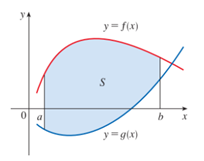
\includegraphics[width=5cm]{area x.png}
                \begin{center}
                    Integration with respect to $x$.
                \end{center}
                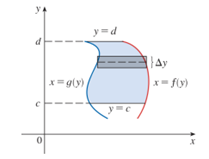
\includegraphics[width=5cm]{area y.png}
                \begin{center}
                    Integration with respect to $y$.
                \end{center}
            \end{multicols}
        \end{center}
    \end{enumerate}
    \hspace*{2em} If the interval of the integration is not provided, try to find the intercept of $f$ and $g$.
    \begin{multicols}{2}
        \textit{\textbf{Example 1}}\\
        The line $y=mx$ cuts the region bounded above by the curve $y=x-x^2$ and below by the $x$-axis into two parts.Then, the areas of the two parts are equal when $m$ is?\\
        \textit{\textbf{Exercise 1}}\\
        Find the values of c such that the area of the region bounded by the parabolas $y=x^2-c^2$ and $y=c^2-x^2$ is $576$.
    \end{multicols}
\newpage

    \item Volume\\
    \hspace*{2em}Calculating volume can be considered as accumulating small layers of cross-sectional areas until a certain value of height or thickness is reached, the following two pictures demonstrates this idea clearly.
    \begin{center}
        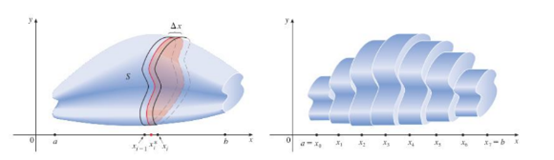
\includegraphics[width=15cm]{V.png}
    \end{center}
    \hspace*{2em}Therefore, the volume can be expressed as following eqaution:
    $$V=\displaystyle\int_a^bA(x)\,dx$$
    \hspace*{2em}Next, we’ll be introducing some common methods to calculate volume using integration, note that similarly, integration of volume can also be done in either x or y direction, depending on the axis of rotation.\\
    \begin{enumerate}[(1)]
        \item Disk Method\\
        \hspace*{2em}Used when calculating volume of one single variable function rotating a specific line.\\
        Rotate around $y=k$:
        $$V=\pi\int_a^b(radius)^2\,dx=\pi\int_a^b[f(x)-k]^2\,dx$$
        Rotate around $x=k$:
        $$V=\pi\int_a^b(radius)^2\,dy=\pi\int_a^b[f(y)-k]^2\,dy$$
    \begin{multicols}{2}
        \textit{\textbf{Example 1}}\\
        Evaluate the volume enclosed by the curves, $x=2\sqrt y$, $x=0$, $y=9$, about $x=0$.\\
        \textit{\textbf{Exercise 1}}\\
        The integral $\displaystyle\int_0^{\frac{\pi}{2}}\pi sin^2*(x)\,dx$ represents the volume of a solid, describe the solid.
    \end{multicols}
\newpage        
        \item Washer Method\\
        \hspace*{2em}Used when calculating volume between two single variable functions, we choose the area enclosed by two curves $f(x)$ and $g(x)$, then rotate around a specific line.\\
        \hspace*{2em}Let’s say we rotate around $y$-axis, then the volume will be:
        $$V=\pi\int_a^bR^2(x)-r^2(x)\,dx$$
        \hspace*{2em}If we rotate around $y=k$, then the volume will be:
        $$V=\pi\int_a^b[R(x)-k]^2-[r(x)-k]^2\,dx$$
        \begin{multicols}{2}
            \textit{\textbf{Example 1}}\\
            The base of solid $S$ is a circular disk with radius $r$.\\Parallel cross-sections prependecular to the base are squares. Find the volume of $S$.\\
            \textit{\textbf{Exercise 1}}\\
            Find the volume common to two spheres, each with radius $r$, if the center of each sphere lies on the\\
            surface of the other sphere.
        \end{multicols}
\newpage        
        \item Cylindrical Shell Method\\
        \hspace*{2em}Cylindrical Methods is dividing the solid bodies into several cylinders, and calculate the volume of the solid bodies by sum up the volume of cylinders.\\
        \hspace*{2em}We can list the general equation for this method:
        $$V=\int_{r_1}^{r_2}2\pi r\cdot h(r)\cdot dr$$
    \end{enumerate}
    \begin{center}
        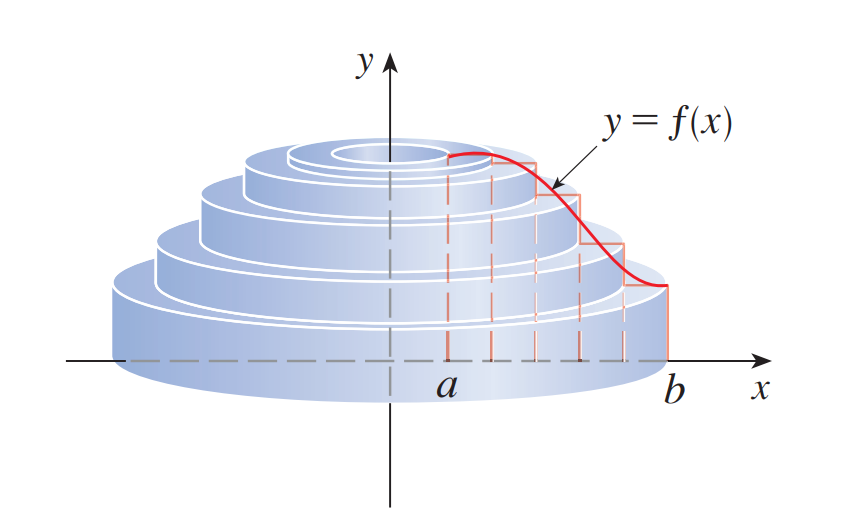
\includegraphics[width=8cm]{cylinder.png}
    \end{center}\leavevmode
    Find the volume generated by rotating the region bounded by the given curves about the specified axis.
    \begin{multicols}{2}
        \textit{\textbf{Example 1}}\\
        $x=2y^2$, $y\geq0$, $x=2$; about $y=2$.\\
        \textit{\textbf{Exercise 1}}\\
        $x=(y-1)^2$, $x-y=1$; about $x=-1$.
    \end{multicols}
\newpage
\item Arc Length
\begin{enumerate}[(1)]
    \item The Arc Length of the Formula\\
    \hspace*{2em}The arc length formula is used to calculate the arc length of a specific function which has a definite range of x.
    $$\text{If}\ f'\ \text{is continuous on}\ [a,b]\text{, and the curve}\ y=f(x),\ a\leq x\geq b$$
    $$\text{Arc Length} = \int_a^b \sqrt{1+[f'(x)]^2}dx$$
    \item The Arc Length Function\\
    \hspace*{2em}Obviously, the arc length function will be used when calculating the arc length of a specific function which doesn’t have a definite range of x, in other words, it measures the arc length starting from a specific point to any other point on the curve.
    $$\text{If}\ f'\ \text{is continuous on}\ [a,b]\text{, and the curve}\ y=f(x),\ a\leq x\leq b$$
    $$\text{Arc Length}=s(x)=\int_a^x\sqrt{1+[f'(x)]^2}dx$$
    \hspace*{2em}Since the function above is an integrating function, it can therefore be transformed into a differential equation by the F.T.C., which is:
    $$\frac{d}{dx}s(x)=\sqrt{1+[f'(x)]^2}$$
    $$ds=\sqrt{1+(\frac{dy}{dx})^2}\,dx\text{ or }ds=\sqrt{1+(\frac{dx}{dy})^2}\,dy\text{ or }ds=\sqrt{(dx)^2+(dy)^2}$$
\end{enumerate}
    \begin{multicols}{2}
        \textit{\textbf{Example 1}}\\
        Find the length of the curve $y=\int_1^x\sqrt{t^3-1}\,dt,\\ 1\leq x\leq 4$\\
        \textit{\textbf{Exercise 1}}\\
        Find the arc length function of the curve \\
        $y=sin^{-1}x+\sqrt{1-x^2}$ with starting point $(0,1)$.
    \end{multicols}
\newpage
\item Area of a Surface of Revolution\\
If $f$ has continuous derivative and $y=f(x),\ a\leq x\leq b\  \equiv\ x=g(y),\ c\leq x\leq d$.
\begin{enumerate}[(1)]
    \item Rotate $y=f(x)$ around $y=c$.\\
    \begin{align}
        \nonumber S=&\int_a^b2\pi r(x)\,ds\\ \nonumber
        =&\int_a^b2\pi |f(x)-c|\sqrt{1+[f'(x)]^2}\,dx\\ \nonumber 
        =&\int_c^d2\pi |y-c|\sqrt{1+[g'(y)]^2}\,dy
    \end{align}
    \item Rotate $x=g(y)$ around $x=c$.\\
    \begin{align}
        \nonumber S=&\int_a^b2\pi r(x)\,ds\\ \nonumber
        =&\int_c^d2\pi |g(y)-c|\sqrt{1+[g'(y)]^2}\,dy\\ \nonumber 
        =&\int_a^b2\pi |x-c|\sqrt{1+[f'(x)]^2}\,dx
    \end{align}
\end{enumerate}
\begin{multicols}{2}
    \textit{\textbf{Example 1}}\\
    The curve $y=\sqrt{r^2-x^2},\ -r\leq x\leq r$,
    is an arc of the circle $x^2+y^2=r^2$.
    Find the area of the surface by rotating this arc about the $x$-axis.\\
    \textit{\textbf{Exercise 1}}\\
    Find the area of the surface generated by\\
    revolving the curve $x=\frac{e^y+e^{-y}}{2}$,
    where $0\leq y\leq ln(2)$, about the $y$-axis.
\end{multicols}
\end{enumerate}
\end{document}